\documentclass[a4paper]{article}

\addtolength{\hoffset}{-2.25cm}
\addtolength{\textwidth}{4.5cm}
\addtolength{\voffset}{-3.25cm}
\addtolength{\textheight}{5cm}
\setlength{\parskip}{0pt}
\setlength{\parindent}{0in}

%----------------------------------------------------------------------------------------
%	PACKAGES AND OTHER DOCUMENT CONFIGURATIONS
%----------------------------------------------------------------------------------------

\usepackage{blindtext} % Package to generate dummy text
\usepackage{charter} % Use the Charter font
\usepackage[utf8]{inputenc} % Use UTF-8 encoding
\usepackage{microtype} % Slightly tweak font spacing for aesthetics
\usepackage[english]{babel} % Language hyphenation and typographical rules
\usepackage{amsthm, amsmath, amssymb} % Mathematical typesetting
\usepackage{float} % Improved interface for floating objects
\usepackage[final, colorlinks = true,
            linkcolor = black,
            citecolor = black]{hyperref} % For hyperlinks in the PDF
\usepackage{graphicx, multicol} % Enhanced support for graphics
\usepackage{xcolor} % Driver-independent color extensions
\usepackage{marvosym, wasysym} % More symbols
\usepackage{rotating} % Rotation tools
\usepackage{censor} % Facilities for controlling restricted text
\usepackage{listings} % Environment for non-formatted code, !uses style file!
\usepackage{pseudocode} % Environment for specifying algorithms in a natural way
 % Environment for f-structures, !uses style file!
\usepackage{booktabs} % Enhances quality of tables
\usepackage{tikz-qtree} % Easy tree drawing tool
 % Configuration for b-trees and b+-trees, !uses style file!
\usepackage[backend=biber,style=numeric,
            sorting=nyt]{biblatex} % Complete reimplementation of bibliographic facilities
\addbibresource{ecl.bib}
\usepackage{csquotes} % Context sensitive quotation facilities
\usepackage[yyyymmdd]{datetime} % Uses YEAR-MONTH-DAY format for dates
\renewcommand{\dateseparator}{-} % Sets dateseparator to '-'
\usepackage{fancyhdr} % Headers and footers
\pagestyle{fancy} % All pages have headers and footers
\fancyhead{}\renewcommand{\headrulewidth}{0pt} % Blank out the default header
\fancyfoot[L]{} % Custom footer text
\fancyfoot[C]{} % Custom footer text
\fancyfoot[R]{\thepage} % Custom footer text
\newcommand{\note}[1]{\marginpar{\scriptsize \textcolor{red}{#1}}} % Enables comments in red on margin
\usepackage{mathtools}
\usepackage{amsmath}
\DeclarePairedDelimiter\abs{\lvert}{\rvert}%
\usepackage{cancel}
\usepackage{minted}
\usepackage{float}
\usepackage{caption}
\usepackage{subcaption}
%-------------------------------

%----------------------------------------------------------------------------------------

%-------------------------------
%	ENVIRONMENT SECTION
%-------------------------------
\pagestyle{fancy}
\usepackage{mdframed}

\usepackage[sfdefault]{FiraSans} %% option 'sfdefault' activates Fira Sans as the default text font
\usepackage[T1]{fontenc}
\renewcommand*\oldstylenums[1]{{\firaoldstyle #1}}


% remove numbering from sections
\usepackage{titlesec}
\titleformat{\section}{\normalfont\Large\bfseries}{}{0pt}{}



%-------------------------------------------------------------------------------------------
%	CUSTOM COMMANDS
%-------------------------------
\newcommand{\gaussian}{\frac{1}{\sigma\sqrt{2\pi}}\exp\left(- \frac{(x-\mu)^2}{2\sigma^2}\right)}
\newcommand{\R}{\mathbb R}

\def\inline{\lstinline[basicstyle=\ttfamily,keywordstyle={}]}


\begin{document}


%-------------------------------
%	TITLE SECTION
%-------------------------------

\fancyhead[C]{}
\hrule \medskip % Upper rule
\begin{minipage}{0.295\textwidth}
\raggedright
\footnotesize
Francisco Javier Sáez Maldonado \hfill\\
franciscojavier.saez@estudiante.uam.es
\hfill\\
\end{minipage}
\begin{minipage}{0.4\textwidth}
\centering
\large
Face Recognition Lab Report\\
\normalsize
Deep Learning for Biometric Signal Processing\\
\end{minipage}
\begin{minipage}{0.295\textwidth}
\raggedleft
\today\hfill\\
\end{minipage}
\medskip\hrule

%-------------------------------
%	CONTENTS
%-------------------------------
\section{Task 1}

Based on the provided code, run the “FaceRecognition.m” file and complete the following points.

\subsection{Paste one image of the ATT Face Dataset and the corresponding image after using the 2D Discrete Cosine Transform (DCT)}

Firstly, I randomly changed the pre-set image to load and show. The one selected was the one shown in Figure \ref{fig:ex1a}


\begin{figure}[H]
  \centering
       \begin{subfigure}[t]{0.45\textwidth}
         \centering
         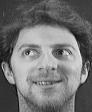
\includegraphics{Figures/Original}
         \caption{Original Image: \emph{s07/3.pgm}.}
     \end{subfigure}%
     \quad
     \begin{subfigure}[t]{0.45\textwidth}
         \centering
         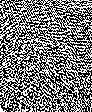
\includegraphics{Figures/Original-DCT}
         \caption{DCT applied to original image.}
     \end{subfigure}
    \caption{Original face and DCT applied to it.}
    \label{fig:ex1a}
\end{figure}

The image on the right is a representation of the image on the left. This representation si created using the \textbf{Discrete cosine transform}, that is, using sums of \emph{cosines}. There are a few different ways of expressing the DCT, but one of the most common ones is:
\[
 X_{k}=\sum _{n=0}^{N-1}x_{n}\cos \left[\,{\tfrac {\,\pi \,}{N}}\left(n+{\frac {1}{2}}\right)k\,\right]\qquad {\text{ for }}~k=0,\ \dots \ N-1
\]

\subsection{Using the original configuration parameters (\inline{train = 6} images, \inline{test = 4} images, DCT \inline{coefficients = 10}), plot the resulting DET image and indicate the resulting EER.}

We only have to let the whole \inline{FaceRecognition.m} script to execute. At the end, it plots the \emph{DET (Detection Error Trade-Off)} curve, which is a compromise between a False Rejection Rate (\emph{(FRR)}) and a False Acceptance Rate (\emph{FAR}). 

The \textbf{EER} is the point where \(FAR = FRR\), that is, the point where we accept the same percentage of false examples that we reject of positive examples. It is marked with a circle in Figure \ref{fig:ex1b}


\begin{figure}[H]
  \centering
  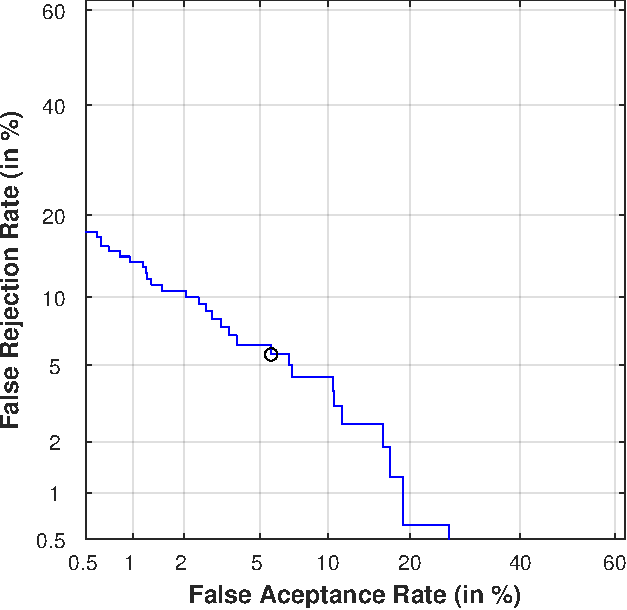
\includegraphics[scale=0.7]{Figures/EER-1}
    \caption{DET curve with marked EER.}
    \label{fig:ex1b}
\end{figure}

We can appretiate in Figure \ref{fig:ex1b} that the EER (circled) is around \(\sim 5.5\%\). Also, the code shows on screen that the EER is \inline{EER = 5.6571}.


\subsection{Find out the configuration of the DCT coefficients that achieves the best EER results (keeping train = 6 images, test = 4 images). Justify your result, including the resulting DET image and EER value.}

In this case where the number of images is small and the techniques that we apply to the image do not take long to execute, we can perform a \emph{grid search} varying the \emph{coefficients} parameter. We have done the following steps:

\begin{enumerate}

\item Extracted the important parts of the code file \inline{FaceRecognition.m} and introduced them in a new file (\inline{eer.m}) containing the function \inline{eer(n_train,n_test,param_coeff)} that, given the number of images used for train and test, and given a number of coefficients, computes the EER for those parameters.
  
\item We have created the script \inline{grid_search_coeff} that executes the code in \inline{eer.m} using the range \(\{1,\dots,20\}\) for the coefficients and saving the EER result in each case.

\item We plot the results in a chart, remarking the minimum. this is shown in Figure \ref{fig:ex1c}.
\end{enumerate}

\begin{figure}[H]
  \centering
  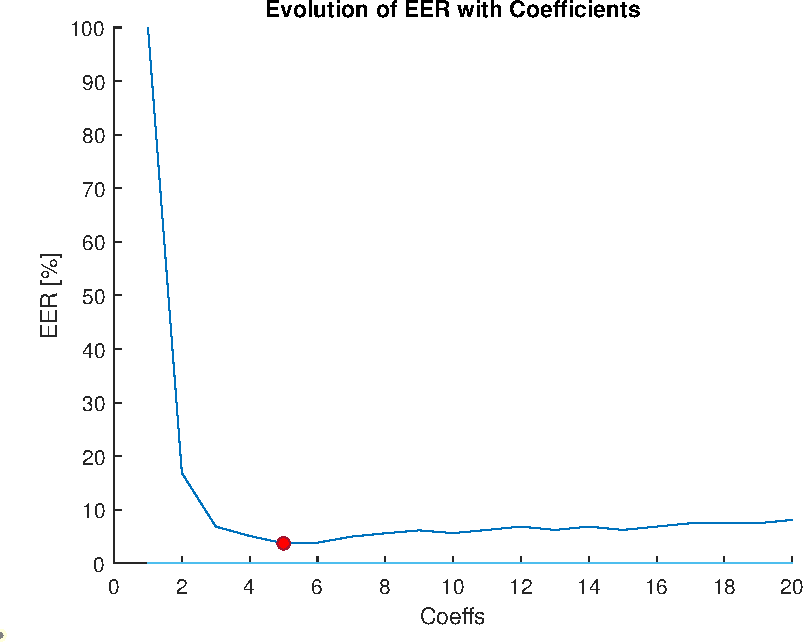
\includegraphics[scale=0.5]{Figures/EERvsCOEFF}
    \caption{Evolution of the EER with the number of coefficients.}
    \label{fig:ex1c}
\end{figure}


As we can see, the \textbf{optimal} number of coefficients is \(5\), obtaining an \(EER = 3.750\). We can appretiate how using a small number of coefficients, the EER is very high (the features are not captured). When using more than \(5\), the EER slowly starts to increase.


\subsection{ Once selected the best configuration of the DCT coefficients (in previous point), analyze the influence of the number of training images in the system performance. Include the EER result achieved for each case (from \(train = 1\) to \(train = 7\)). Justify the results.}


In this case, we can make good use of our previously defined function \inline{eer} and adapt the code in \inline{grid_search_coeff} to make it vary the parameter \inline{n_train} (and, thus, \inline{n_test} since \(n\_test = total - n\_train\)).

We create a new script called \inline{grid_search_ntrain} that uses \(n\_train = \{1,\dots,9\}\) and we run the script, obtaining the graph in Figure 

\begin{figure}[H]
  \centering
  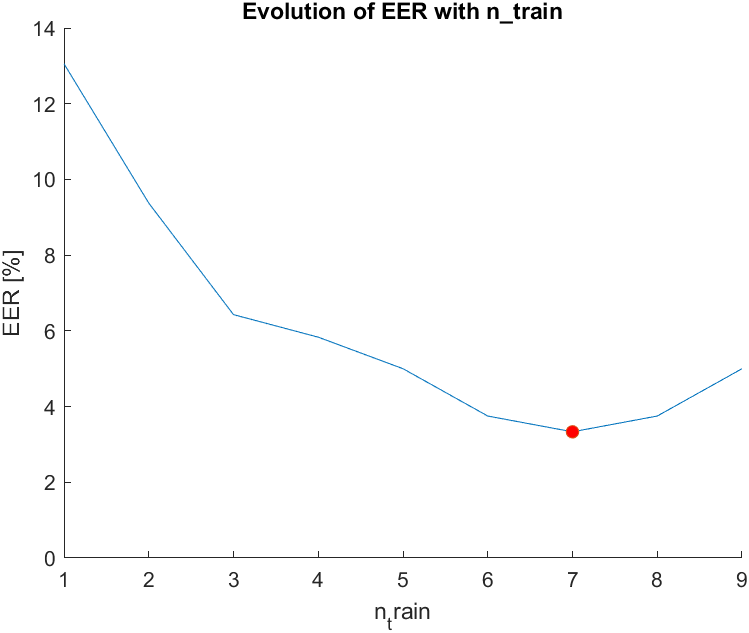
\includegraphics[scale=0.5]{Figures/EERvsNTRAIN}
    \caption{Evolution of the EER with the number of coefficients.}
    \label{fig:ex1d}
\end{figure}

The minimum value of the EER is obtained when we use \(n\_train = 7\) images, obtaining \(EER = 3.33\), which is a lower value than the one we obtained previously when we optimized the coefficients.\\ 


With this and the previous question, what we have done is typically called \textbf{grid search}, that is, searching for the best hyperparameters of our model. Usually, the number of images in train and test subsets is not an hyperparameter, since the quantity of available images is much higher, and a partition of \(70-75\%\) of the size is chosen for train and the rest for the test set. In this case, we reached that the train set has the \(70\%\) of the total size of our dataset. 

The results are positive, since we have searched for the combination that \textbf{optimizes} the EER in this particular problem. As a quick recall, the optimal parameters when we seek to \textbf{minimize the EER} are:
\begin{enumerate}
\item \(n\_train = 7, n\_test = 3\)
\item \(coefficients = 5\)
\end{enumerate}


\section{Task 2}
The goal of this task is to change the feature extraction module. Instead of using DCT coefficients as in Task 1, you must consider Principal Component Analysis (PCA) to extract more robust features. 
You can use the pca.m function available in Matlab. For the training phase, you should follow:
\begin{minted}{MatLab}
[coeff_PCA,MatrixTrainPCAFeats,latent] = pca(MatrixTrainFeats);
meanTrainMatrix=mean(MatrixTrainFeats);
\end{minted}
It is important to remark that the PCA function must be applied once for all training users and samples (not one PCA per user as this would provide specific \inline{coeff_PCA} parameters per user).  
For the test phase, you should follow:
\begin{quote}
For each test, subtract the meanTrainMatrix, and multiply by the \inline{coeff_PCA} transformation matrix in order to obtain the test features in the PCA domain.
\end{quote}
For more information, check Matlab Help: \url{https://es.mathworks.com/help/stats/pca.html}

\subsection*{Preparation}

\textbf{Note.-} The code of this preparation section can be found in the file \inline{PCA_EER.m}.\\

To begin with this task, we must adapt the code used before in order to change the way the feature extraction is done. We are told that we must apply PCA as it is usually done: to a \(M \in \mathcal M_{r \times c}\) matrix with \(r\) examples with \(c\) features per example. The idea is to reduce that matrix to another matrix \(M_{PC} \in \mathcal M_{r \times c'}\), where \(r' < r\), but keeping the most relevant information about each image.

Thus, we change the way we store the images, we now \emph{flatten} each of them into a single row to create the just mentioned \(M\) matrix. We declare in this case a Matrix of size \(Train\cdot 40 \times  (image\_length \cdot image\_width)\).

\begin{minted}{MatLab}
  size = length*width;
  %Initialize the Feature and Label Matrix for both train and test
  MatrixTrainFeats=zeros(Train*40,size); 
  MatrixTestFeats=zeros(Test*40,size); 
\end{minted}

Then, we have to flatten (convert each image matrix \(M \in \mathcal M_{r \times c}\) to a vector in \(\mathbb R^{r \cdot c}\), and introduce in the corresponding \emph{Train/Test Matrix}. We have slightly changed how the code of the original \inline{FaceRecognition.m} does this part, making it a little bit easier. The result is the following:

\begin{minted}{MatLab}
  for j=1:10
  im=imread(images(j).name);
  im=double(im);
  % Flatten image and add it to big matrix
  im_flat = reshape(im.',1,[]);

  %%%  Training Dataset
  if j <= Train
      MatrixTrainFeats((i-1)*Train + j, : ) = im_flat;
      MatrixTrainLabels((i-1)*Train + j, 1) = i;
  %%% Test dataset
  else
      MatrixTestFeats((i-1)*Test + (j - Train), : ) = im_flat;
      MatrixTestLabels((i-1)*Test + (j - Train), 1) = i;
  end
\end{minted}

Lastly, as we are indicated in the task, we have to extract the principal components of the matrix that contains the features of \textbf{all} the images, that is: \inline{MatrixTrainFeats}. The MatLab method \inline{pca} returns the mean \(\mu\) and the PCA coefficients, so we can use them to project the Test set into the feature space.
\begin{minted}{MatLab}
  % PCA on Training matrix
  [PCA_coeffs,MatrixTrainPCA,latent,none,explained,mu] = pca(MatrixTrainFeats);
  % Project Test Set
  MatrixTestPCA = (MatrixTestFeats - mu)*PCA_coeffs;  
\end{minted}

We remark the information contained in each of the returned variables from PCA:

\begin{itemize}
\item \inline{PCA_coeffs}\(\in \mathcal M_{p \times p}\) are the coefficients of the principal components.
\item \inline{MatrixTrainPCA} contains the representation of the original data in the principal component feature space.
\item \inline{latent} contains the  Hotelling's T-squared statistic for each observation in X.
\item \inline{explained} contains the percentage of the total variance explained by each principal component.
\item \inline{mu} contains the estimated mean of each variable in the original data.
\end{itemize}

The distance computation used in \inline{FaceRecognition.m} is kept, so we do not modify it. We are now ready to perform the required sub-tasks.

\subsection{ Using the parameters \(train = 6\) and \(test = 4\), paste the DET curve and indicate the EER when using all the PCA components.}


Using the previously commented code, we run the \inline{PCA_EER} script with the mentioned sizes for train and test subsets and obtain the DET curve plotted in Figure \ref{fig:ex2a}. In this subtask, we use \textbf{all components} obtained by PCA.

\begin{figure}[H]
  \centering
  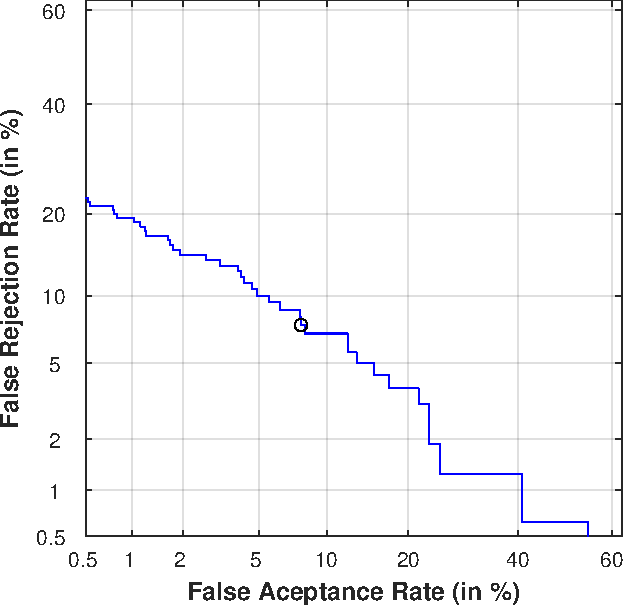
\includegraphics[scale=0.7]{Figures/PCA-1-EER}
    \caption{DET curve for PCA with \(n\_train = 6\) and \(n\_test = 4\), using \textbf{all components}.}
    \label{fig:ex2a}
\end{figure}

We obtain an \(EER = 8.0769\), which is approximately \(2.5 \%\) higher than the one we obtained in the simplest case using the DCT. Using all the components returned from PCA is not the best option.



\subsection{ A key aspect for the PCA is the number of components considered. Analyze and represent how the EER value changes in terms of the number of PCA components. Give your explanation about the results achieved.}

As we already know, we obtain the principal components by diagonalizing the covariance matrix of the data. This way, we obtain principal directions \(v_1,\dots, v_n\) and eigenvalues \(\lambda_1,\dots,\lambda_n\), which indicate the \textbf{percentage} of the variance explained by each component. The components are sorted by the variance explained (its eigenvalue \(\lambda_i\). The most common technique when using PCA is \textbf{selecting} a number of components that explain a decent amount of the variance. 

In order to determine how many components we want to select, let us first do an analysis of the variance explained. We find (by obtaining the number of elements of the variable \inline{explained}) that PCA returns \(239\) components. Let us show in Figure \ref{fig:ex2b}  the percentage of variance explained by each of them and the accumulated variance explained by the components \(1,\dots, i\) for each \(i = 1,\dots, 239\). 

\begin{figure}[H]
  \centering
       \begin{subfigure}[t]{0.45\textwidth}
         \centering
         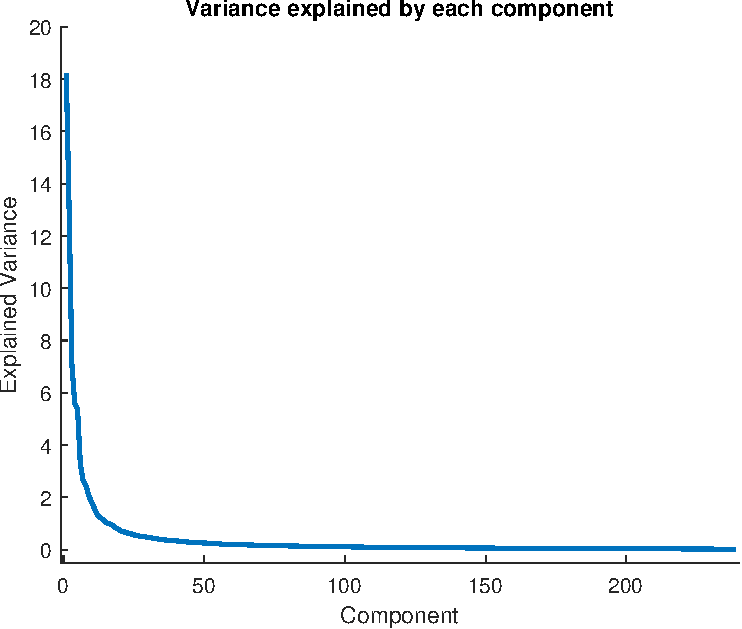
\includegraphics[scale=0.6]{Figures/VariancePerComponent}
         \caption{Variance explained by each component.}
     \end{subfigure}%
     \quad
     \begin{subfigure}[t]{0.45\textwidth}
         \centering
         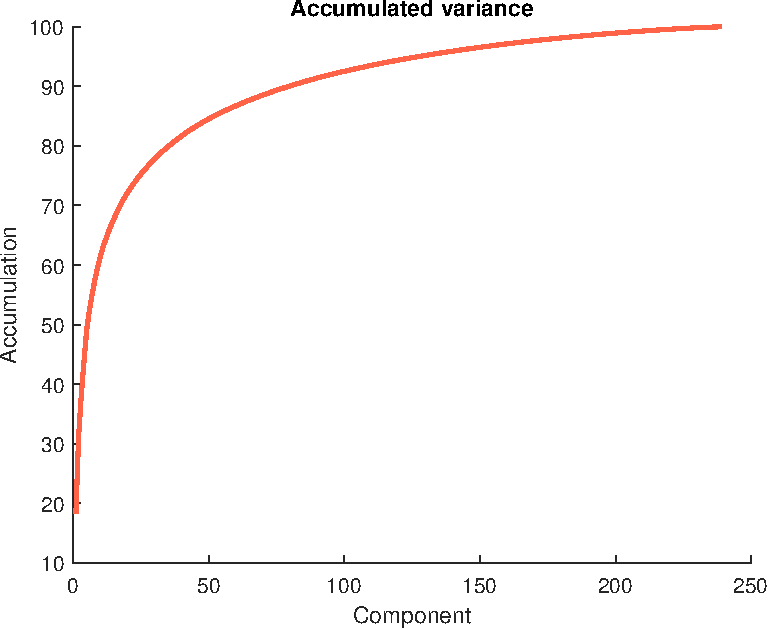
\includegraphics[scale=0.6]{Figures/accumulated_variance}
         \caption{Accumulated variance explained.}
     \end{subfigure}
    \caption{Explained variance representations.}
    \label{fig:ex2b}
\end{figure}

We can observe in the graphics that using approximately \(50\) components we are explaining \(\approx 80\%\) of the total variance, which is usually enough to be able to classify the images well. Also, from the component \(50\) onwards, the components explain less than \(1\%\) of the total variance, which means that they are possibly not really relevant.\\

We now compute the EER for each number of components. There is a little adaptation that the current code 


\subsection{ Indicate the optimal number of PCA components and paste the resulting DET curve together with the EER achieved. Compare the results using PCA with the DCT features considered in Task 1.}




\section{Extra Task}

The goal of this task is to improve the matching module. Instead of using a simple distance comparison, you must consider Support Vector Machines (SVM). In this case, you should train one specific SVM model per user using the training data (train = 6 images).
Features extracted using the PCA module developed in Task 2 must be considered in this Task. 
You can use the fitcsvm function available in Matlab. For the training phase, you should follow:
\begin{minted}{MatLab}
SVMModel = fitcsvm(…)
\end{minted}
For the test phase, you should follow:
\begin{minted}{MatLab}
[label,score]= predict(SVMModel,MatrixTestFeats);
\end{minted}
to obtain the scores for each user model. 
For more information, check Matlab Help:
\url{https://es.mathworks.com/help/stats/fitcsvm.html?lang=en} 
\subsection{ Using the parameters train = 6 and test = 4, paste the DET curves and indicate the EERs in the following cases: 1) regarding the KernelFunction parameter of the SVM (using all PCA components), and 2) regarding the number of PCA components considered for the feature extraction module (using the KernelFunction polynomial and starting with 3 PCA components).}




















\end{document}